%! Suppress = MultipleIncludes
\documentclass[tikz,crop]{standalone}

% Part of the preamble, for TikZ figures.
% This is used in both the main document and in the subfigures.
% One exception is minted: since the path depends on the file, it is not set.
\usepackage{tikz}
\usepackage{xcolor}
\usepackage{pgfplots}

\pgfplotsset{compat=1.18}
\usepgfplotslibrary{statistics}

\usetikzlibrary{shapes,arrows,positioning,backgrounds,calc,intersections,calc}

\definecolor{ugent-re}{RGB}{220, 78, 40}        % vermilion			/ vermiljoen
\definecolor{ugent-we}{RGB}{45, 140, 168}       % no match
\definecolor{ugent-ge}{RGB}{232, 94, 113}       % rose				/ bleekrood
\definecolor{ugent-ea}{RGB}{111, 113, 185}      % distant blue		/ verblauw
\definecolor{ugent-pp}{RGB}{251, 126, 58}       % deep orange		/ dieporanje
\definecolor{ugent-ps}{RGB}{113, 168, 96}       % yellow green		/ geelgroen

\tikzstyle{python}=[fill=ugent-ps!50!white]
\tikzstyle{java}=[fill=ugent-we!50!white]
\tikzstyle{haskell}=[fill=ugent-ea!50!white]
\tikzstyle{js}=[fill=ugent-pp!50!white]
\tikzstyle{c}=[fill=ugent-re!50!white]

\newlength{\block}
\setlength{\block}{0.75cm}

\tikzstyle{a}=[anchor=north west]
\tikzstyle{box}=[a,draw,rectangle]
\tikzstyle{node}=[a,draw,minimum height=0.5cm,align=center,fill=white,text depth=.25ex]
\tikzstyle{document}=[node,tape,tape bend top=none]
\tikzstyle{cont}=[box,minimum height=1\block,minimum width=1\block]
\tikzstyle{arrow}=[draw, -latex]
\tikzstyle{inner}=[box,draw=gray]

% Blue box style
\tikzstyle{bluebox}=[draw=ugent-we,java]
\tikzstyle{redbox}=[draw=ugent-re,c]
\tikzstyle{greenbox}=[draw=ugent-ps,python]

% Some things specific to TESTed imagery.
\tikzstyle{tc}=[box,draw=ugent-ps]
\tikzstyle{comp}=[box,draw=ugent-re,fill=ugent-re,fill opacity=0.05]
\tikzstyle{exec}=[box,draw=ugent-we,fill=ugent-we,fill opacity=0.10]

% Stuff from tested-engine/concept.tex
\tikzstyle{process}=[node,rectangle]
\tikzstyle{terminator}=[node,rectangle,rounded corners=0.5cm]
\tikzstyle{io}=[node,trapezium,trapezium left angle=70,trapezium right angle=-70,minimum width=2.5cm,trapezium stretches=true]
\tikzstyle{small}=[font=\footnotesize,color=darkgray]
\tikzstyle{submission}=[document,align=right,minimum width=3cm,minimum height=1cm,text depth=0.5cm,inner sep=0.5mm,font=\scriptsize]

% Stuff from chatper3/flow.tex
\tikzstyle{height}=[minimum height=0.75\block]
\tikzstyle{contt}=[cont,minimum height=0.75\block]
\tikzstyle{compop}=[comp,text opacity=1]
\tikzstyle{execop}=[exec,text opacity=1]

\tikzstyle{hnode}=[draw,anchor=center,minimum height=\block,text depth=.25ex,align=center]
\tikzstyle{executable}=[hnode,ultra thick,fill=gray!10]
\tikzstyle{inner-exec}=[node,anchor=center,minimum width=3.25\block,densely dotted,font=\footnotesize,fill=none]
\tikzstyle{stmt}=[node,anchor=center,fill=gray!30,minimum width=4.5\block,font=\footnotesize]
\tikzstyle{fieldset}=[minimum height=\block,fill=white,text depth=.5ex,fill=white]

% Minted environments for use in Tikz
\newminted[tikzjava]{java}{autogobble,linenos=false,fontsize=\tiny,stripall}
\newminted[tikzpython]{python}{autogobble,linenos=false,fontsize=\tiny,stripall}
\newminted[tikztext]{text}{autogobble,linenos=false,fontsize=\tiny,stripall}


\begin{document}

\tikzstyle{height}=[minimum height=0.75\unit]
\tikzstyle{contt}=[cont,minimum height=0.75\unit]
\tikzstyle{inner}=[box,draw=gray]
\tikzstyle{arrow}=[draw, -latex]
\tikzstyle{comp}=[draw=ugent-re,fill=ugent-re,fill opacity=0.05,text opacity=1]
\tikzstyle{exec}=[draw=ugent-we,fill=ugent-we,fill opacity=0.10,text opacity=1]

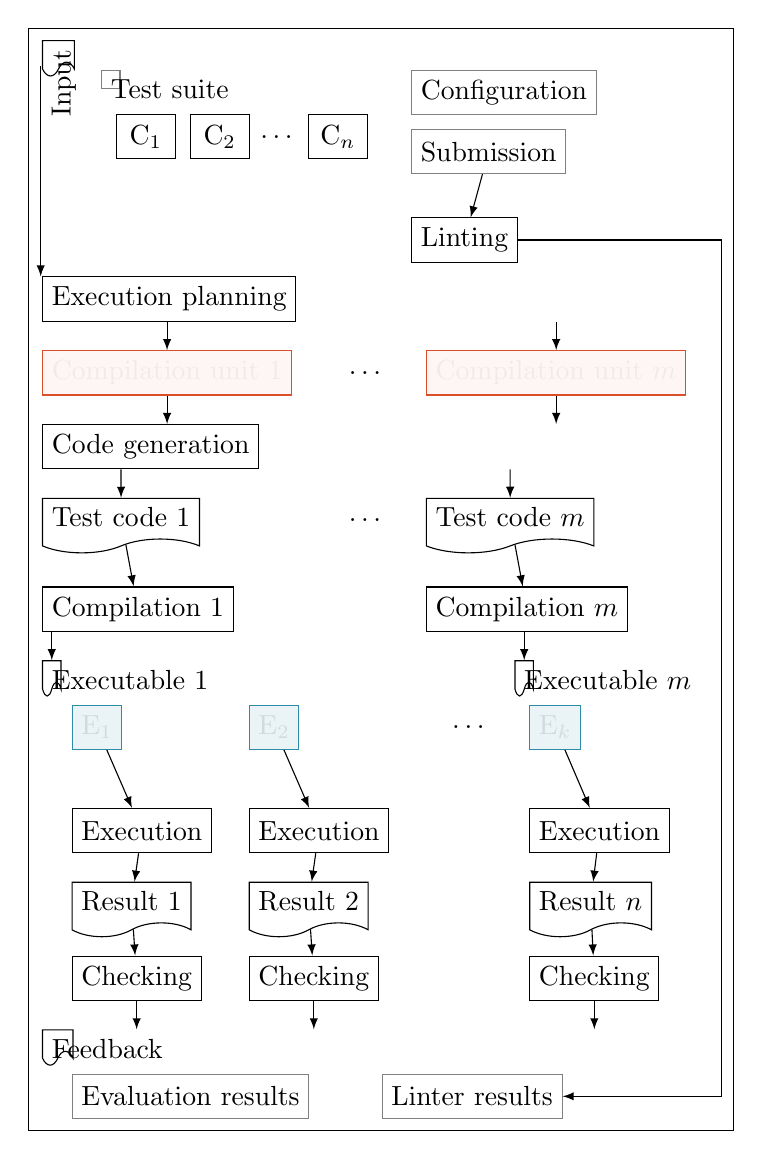
\begin{tikzpicture}[x=0.75cm,y=0.75cm,framed]
%    \draw[step=1,gray!30,thin] (0,0) grid (11,-20);

    \node[document,minimum width=11.5\unit,minimum height=2.75\unit] at (0, 0) (input) {};
    \node[right,rotate=90,anchor=north east] at (input.north west) {Input};

    \node[inner,minimum width=4.75\unit,minimum height=1.75\unit] at (1,-0.5) (tp) {};
    \node[below right] at (tp.north west) {Test suite};
    \node[contt] at (1.25, -1.25) (c1) {C\textsubscript{1}};
    \node[contt] at (2.5, -1.25) (c2) {C\textsubscript{2}};
    \node[contt,draw opacity=0] at (3.5, -1.25) (c2) {\ldots};
    \node[contt] at (4.5, -1.25) (c3) {C\textsubscript{$n$}};

    \node[inner,minimum width=4.75\unit,height] at (6.25,-0.50) (conf) {Configuration};
    \node[inner,minimum width=4.75\unit,height] at (6.25,-1.50) (subm) {Submission};

    \node[box,minimum width=4.75\unit,height] at (6.25,-3) (lint) {Linting};
    \draw[arrow] (subm) -- (lint);

    \node[box,minimum width=11\unit,height] at (0,-4) (plan) {Execution planning};
    \draw[arrow] (input.219) -- (plan.north-|input.219);

    \node[contt,comp,minimum width=4.5\unit] at (0,-5.25) (cu1) {Compilation unit 1};
    \node[contt,draw opacity=0] at (5, -5.25) {\ldots};
    \node[contt,comp,minimum width=4.5\unit] at (6.5,-5.25) (cu2) {Compilation unit $m$};
    \draw[arrow] (plan.south-|cu1) -- (cu1);
    \draw[arrow] (plan.south-|cu2) -- (cu2);

    \node[box,minimum width=11\unit,height] at (0,-6.50) (gen) {Code generation};
    \draw[arrow] (cu1) -- (cu1|-gen.north);
    \draw[arrow] (cu2) -- (cu2|-gen.north);
    \node[document,minimum width=4.5\unit,minimum height=1\unit] at (0,-7.75) (tc1) {Test code 1};
    \node[contt,draw opacity=0] at (5, -7.75) {\ldots};
    \node[document,minimum width=4.5\unit,minimum height=1\unit] at (6.5,-7.75) (tc3) {Test code $m$};
    \draw[arrow] (gen.south-|tc1) -- (tc1);
    \draw[arrow] (gen.south-|tc3) -- (tc3);

    \node[box,minimum width=4.5\unit,height=1] at (0,-9.25) (comp1) {Compilation 1};
    \node[box,minimum width=4.5\unit,height=1] at (6.5,-9.25) (comp2) {Compilation $m$};
    \draw[arrow] (tc1) -- (comp1);
    \draw[arrow] (tc3) -- (comp2);

    \node[document,minimum width=6.5\unit,minimum height=2\unit] at (0, -10.5) (ex1) {};
    \node[below right] at (ex1.north west) {Executable 1};
    \node[document,minimum width=3\unit,minimum height=2\unit] at (8, -10.5) (ex3) {};
    \node[below right] at (ex3.north west) {Executable $m$};
    \draw[arrow] (comp1.south-|ex1) -- (ex1);
    \draw[arrow] (comp2.south-|ex3) -- (ex3);

    \node[box,exec,minimum width=2.5\unit,height] at (0.5,-11.25) (e1) {E\textsubscript{1}};
    \node[box,exec,minimum width=2.5\unit,height=] at (3.5,-11.25) (e2) {E\textsubscript{2}};
    \node[contt,draw opacity=0] at (6.75, -11.25) {\ldots};
    \node[box,exec,minimum width=2.5\unit,height] at (8.25,-11.25) (e3) {E\textsubscript{$k$}};

    \node[box,minimum width=2.5\unit,height=1] at (0.5,-13) (exe1) {Execution};
    \node[box,minimum width=2.5\unit,height=1] at (3.5,-13) (exe2) {Execution};
    \node[box,minimum width=2.5\unit,height=1] at (8.25,-13) (exe3) {Execution};
    \draw[arrow] (e1) -- (exe1);
    \draw[arrow] (e2) -- (exe2);
    \draw[arrow] (e3) -- (exe3);

    \node[document,minimum width=2.5\unit,minimum height=1\unit] at (0.5,-14.25) (res1) {Result 1};
    \node[document,minimum width=2.5\unit,minimum height=1\unit] at (3.5,-14.25) (res2) {Result 2};
    \node[document,minimum width=2.5\unit,minimum height=1\unit] at (8.25,-14.25) (res3) {Result $n$};
    \draw[arrow] (exe1) -- (res1);
    \draw[arrow] (exe2) -- (res2);
    \draw[arrow] (exe3) -- (res3);

    \node[box,minimum width=2.5\unit,height] at (0.5,-15.50) (check1) {Checking};
    \node[box,minimum width=2.5\unit,height] at (3.5,-15.50) (check2) {Checking};
    \node[box,minimum width=2.5\unit,height] at (8.25,-15.50) (check3) {Checking};
    \draw[arrow] (res1) -- (check1);
    \draw[arrow] (res2) -- (check2);
    \draw[arrow] (res3) -- (check3);

    \node[document,minimum width=11\unit,minimum height=2\unit] at (0,-16.75) (fb) {};
    \node[below right] at (fb.north west) {Feedback};
    \draw[arrow] (check1) -- (fb.north-|check1);
    \draw[arrow] (check2) -- (fb.north-|check2);
    \draw[arrow] (check3) -- (fb.north-|check3);

    \node[inner,minimum width=4.75\unit,height] at (0.5,-17.5) (rst) {Evaluation results};
    \node[inner,minimum width=4.75\unit,height] at (5.75,-17.5) (lintres) {Linter results};
    \draw[arrow] (lint) -- (lint-|11.5,) -- (11.5,|-lintres) -- (lintres);

\end{tikzpicture}

\end{document}
